\chapter{Results}
\epigraph{The first law of thermodynamics says that work cannot be destroyed. We who use computers know better.}{A frustrated Ph.D. candidate}

\section{Periodic Orbits}

Four new periodic orbits P85, P60, P32 and P8 (\refFigsss{fig:p85}{fig:p60}{fig:p32}{fig:p8}) have been found, with periods $T= 85.50, 60.86, 32.00, 8.32$, for $\ReN = 400$, and periodic cell length $(\alpha,\gamma) = (2\pi/L_x,2\pi/L_z) = (1.14,1.67)$ with a grid discretization of $(N_x,N_y,N_z) = (48,33,48)$. This  set of cell parameters is known as the HKW cell. P85 and P60 were the first orbits found, and are in the fully symmetric subspace. P32 was the next orbit to be found, and is in the streamwise-asymmetric subspace $S_x$. P8 was the last orbit found, and is in the spanwise-asymmetric subspace $S_z$. I was unable to find any \ecs\ in the unconstrained phase space. 

\begin{figure}
\centerline{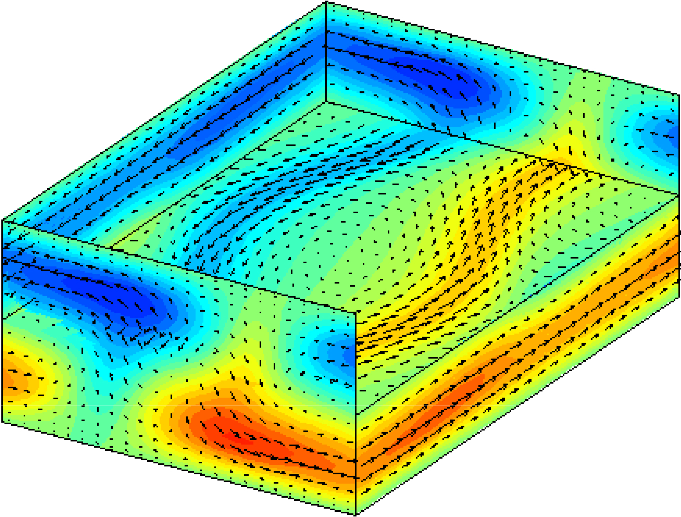
\includegraphics[width=\textwidth]{p85noBase.pdf}}
\caption{P85 is a fully symmetric orbit with period 85.50 in the HKW cell with $\ReN=400$. Note the extreme symmetry of the prominent streaks visible in the mid-plane. The velocity field pictured here is the turbulent perturbation only, with no laminar flow added.}\label{fig:p85}
\end{figure}

\begin{figure}
\centerline{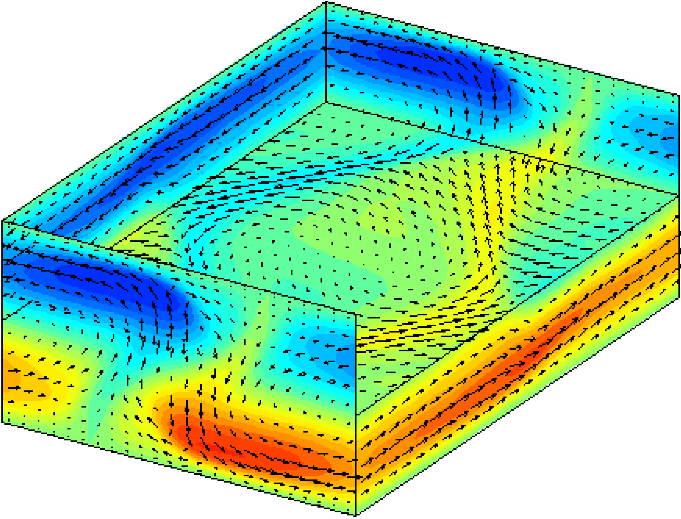
\includegraphics[width=\textwidth]{p60noBase.pdf}}
\caption{P60 is another fully symmetric orbit with period 60.86 in the HKW cell with $\ReN = 400$. While it displays an ellipsoid streak structure similar to P85, the energy of these streaks are lower. The velocity field pictured here is the turbulent perturbation only, with no laminar flow added.}\label{fig:p60}
\end{figure}


\begin{figure}
\centerline{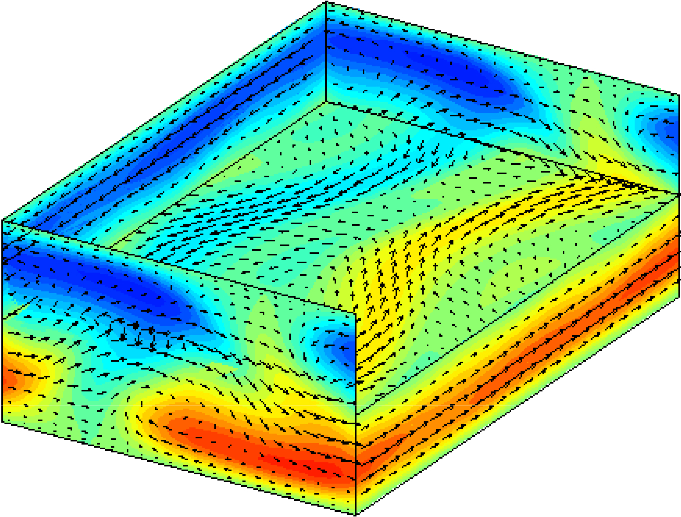
\includegraphics[width=\textwidth]{p32noBase.pdf}}
\caption{P32 is a streamwise asymmetric periodic orbit fixed by the symmetry group $S_z$, which is functionally a mirror symmetry about the streamwise axis. In the HKW cell at $\ReN=400$, the period is 32.00, and the streamwise relative velocity is $-0.5$ cell lengths per period. The velocity field pictured here is the turbulent perturbation only, with no laminar flow added.}\label{fig:p32}
\end{figure}


\begin{figure}
\centerline{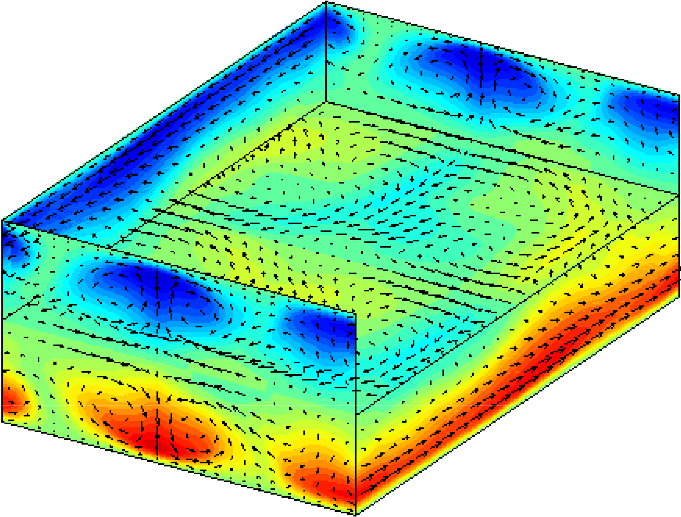
\includegraphics[width=\textwidth]{p8noBase.pdf}}
\caption{P8 is a spanwise asymmetric periodic orbit fixed by the symmetry group $S_x$, which is functionally a rotation by $\pi$ about the spanwise axis. In the HKW cell at $\ReN = 400$, the period is 8.32, and the spanwise relative velocity is $2.29\times 10^{-7}$ cell lengths per period. This number may seem low, but if it is not accounted for, the NKH solver cannot converge. P8 also has a rather low period, almost an order of magnitude lower than most orbits available on {\tt channelflow.org}. Since the Arnoldi iteration has a time cost that scales linearly with the period, P8 has been the least computationally demanding period orbit to analyze.}\label{fig:p8}
\end{figure}

\subsection{Visualizations}   

Visualizing the behavior of fluids is in itself a time-honored discipline, especially when CFD is involved\footnote{As the old joke goes, CFD really stands for {\bf C}olorful {\bf F}luid {\bf D}ynamics.}, and well chosen visualization schemes can be, in and of themselves, an excellent tool for interpreting and analyzing data. We use two main visualization methods here.
\subsubsection{Orthographic Projection}
\refFigsss{fig:p85}{fig:p60}{fig:p32}{fig:p8} are all examples of the first visualization method -- the {\bf orthographic projection} (OP). The OP is constructed by piecing together several representative 2D slices of the state's velocity field -- each of the vertical walls, and the mid-plane, and is colored to represent the magnitude and direction of streamwise velocity. The OP allows us to visually interrogate the structure of the state, which can be extremely useful -- for example, it is clear purely from visual interrogation that \refFig{fig:p8} is less ordered than \refFig{fig:p85}. However, the OP cannot deliver much more than this -- for example, it cannot easily tell us much about the differences between the orbits of, say, P8 and P85. For this reason, we use the second, more useful visualization method - the state space projection.

\begin{figure}[h]
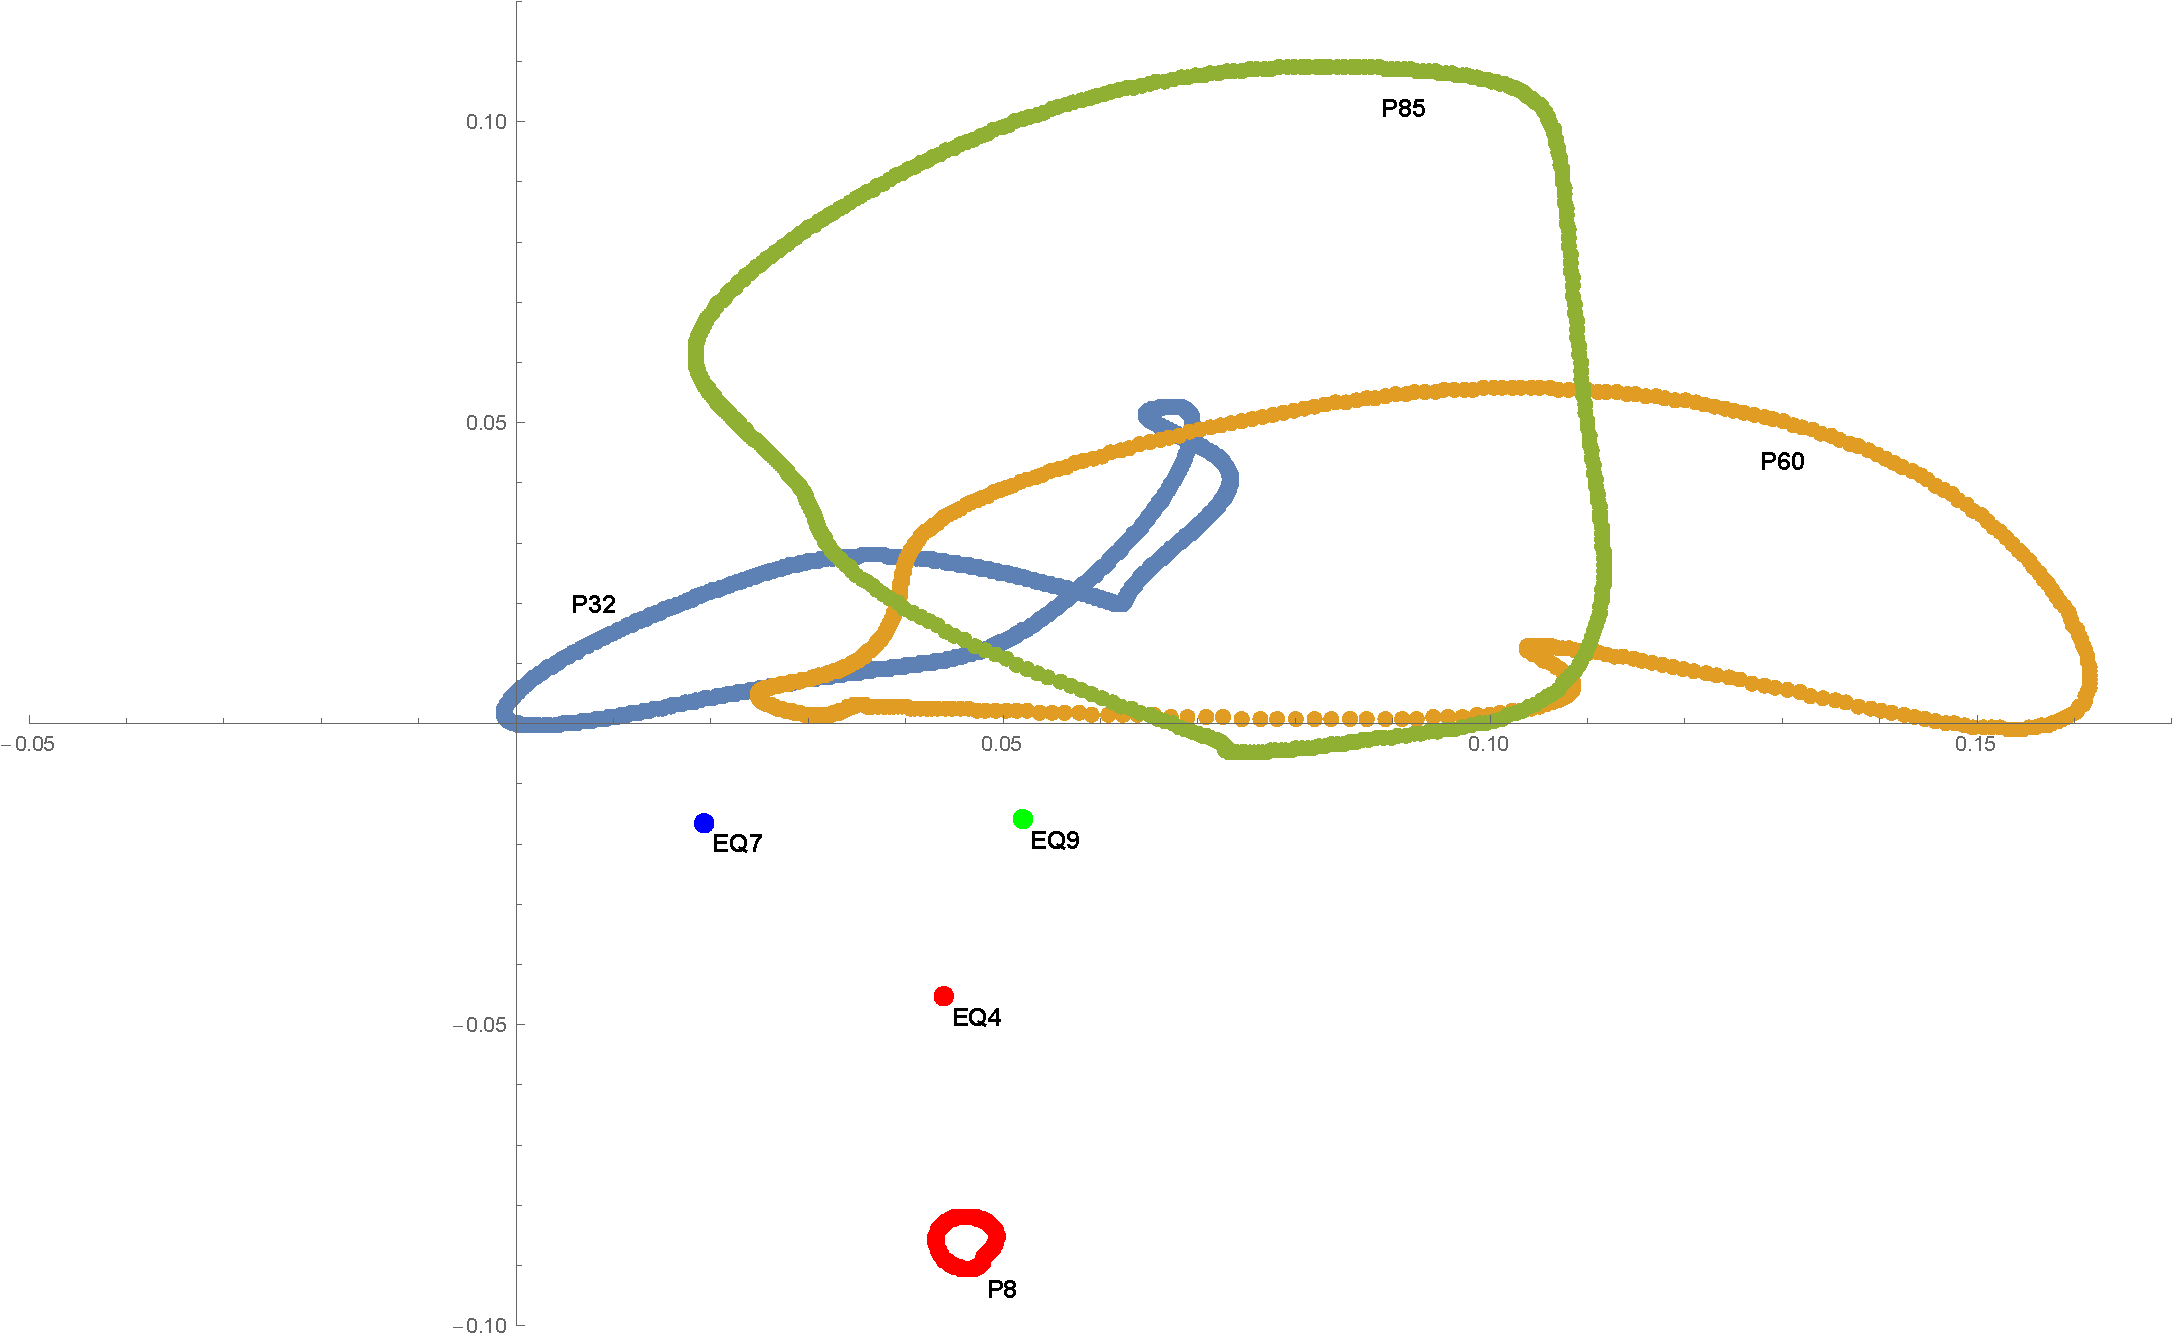
\includegraphics[width=\textwidth]{PeriodicOrbitPO412}
\caption{2D state space projection of all four periodic orbits and some reference equibliria. The basis for the projection was constructed by orthonormalizing the initial states of each of the periodic orbits. The equbiliria are fully symmetric, and were found by\rf{Halcrow2008}. Notice that the P8 orbit is separated by the equilibria from P85, P60 and P32, a feature that holds true in the other 5 projections.}\label{fig:POStateSpace}
\end{figure}

\subsubsection{State Space Projection}
If we have a set of $k$ basis vectors $\Vector{q}_i$ that are orthonormal and span a subspace $\mathfrak{V}_k \subset \mathfrak{V}$ of dimension $k$, then the projection of a vector $\Vector{v} \in \mathfrak{V}$ onto $\mathfrak{V}_k$ is defined 
\begin{equation}
\Vector{v}_k = \sum{i = 1}{k}{c_i \Vector{q}_i},
\end{equation}
where $c_i = \Vector{v} \cdot \Vector{q}_i$. When $k$ is either 2 or 3, we can visualize the $n$-dimensional trajectory as a 2 or 3 dimensional trajectory instead. While we lose information by this projection, we can still gain a great deal of valuable information about trajectories. Projecting the four periodic orbits in \refFigsss{fig:p85}{fig:p60}{fig:p32}{fig:p8} onto a basis constructed from orthonormalizing the initial conditions of each orbit results in the state space projection in \refFig{fig:POStateSpace}. The main issue with the state space projection method, however, is that a state must be {\bf congruent} to a basis to be project - that is, both the box length and grid discretization must be the same for both the state and the projection basis. Many previous results\rf{Gibson2008,Halcrow2008} have results in the W03 cell, where $(\alpha,\gamma) = (1.14,2.5)$, with corresponding state space projections. In order to compare to these results, I attempted to use \refAlg{alg:parCont} to continue the four periodic orbits into the W03 cell, which leads me to the next important result.

\section{Spanwise Continuation}

When \refAlg{alg:parCont} was used to continue P8 down to the W03 cell, the data presented in \refFig{fig:LZBif} was produced.
\begin{figure}[b!]
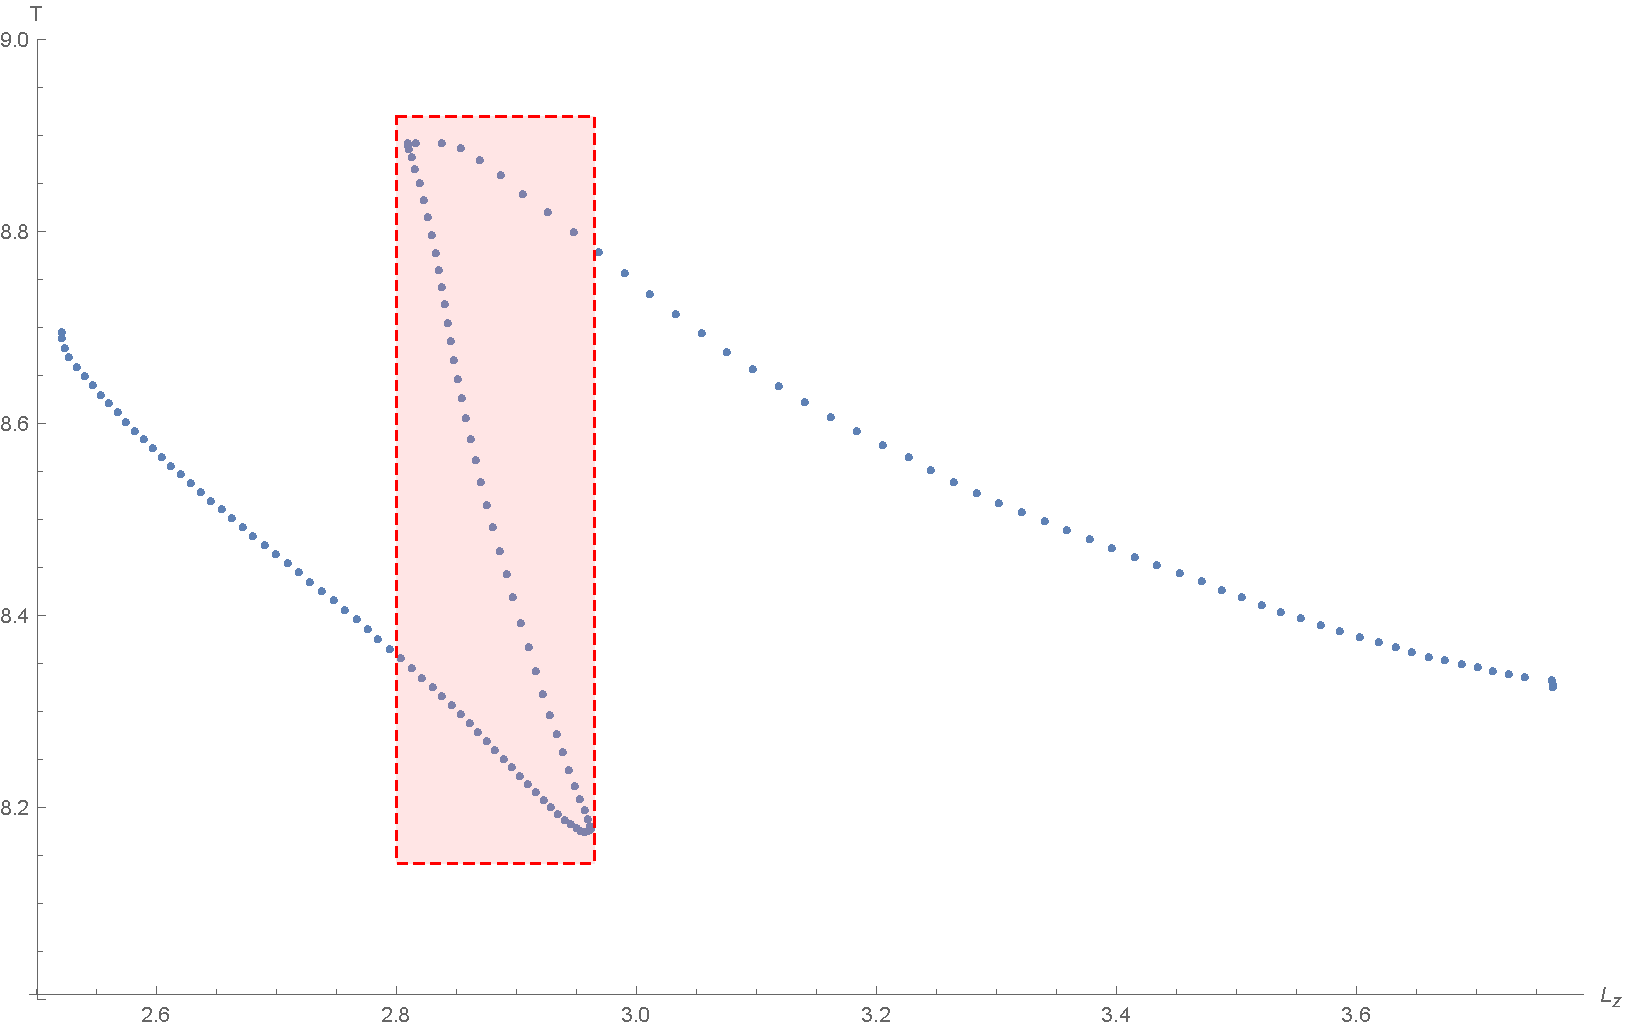
\includegraphics[width=\textwidth]{TLzBD}
\caption{Period as a function of spanwise cell length for P8. Initially, the continuation algorithm decreases $L_z$ and increases $T$, but at $L_z \approx 2.8$, the algorithm reverses itself, decreasing $T$ and increasing $L_z$, until $L_z \approx 2.95$, when the algorithm resumes decreasing $L_z$ and increasing $T$. Since we expect that the period of an orbit ought to uniquely define the orbit, the existence of multiple, distinct orbits for $2.8 \leq L_z \leq 2.96$ hints at a bifurcation.}\label{fig:LZBif}
\end{figure}
\begin{figure}[t]
\includegraphics[width=\textwidth]{phasePortraitTransition}
\caption{Phase portrait of the Van Der Pol oscillator and its Hopf bifurcation, with trajectories in white. (a), for negative values of the bifurcation parameter, the single periodic orbit is unstable, so an initial condition that begins near the orbit spirals away from it. (b), when the bifurcation parameter is zero, there is no periodic orbit. (c), for positive values of the bifurcation parameter, the periodic orbit is stable, and initial conditions are attracted into the orbit.}\label{fig:phasePortrait}
\end{figure}
 Attempts to continue the other three periodic orbits down generally failed, the cause of which is unclear. The similarity of \refFig{fig:LZBif} to \refFig{fig:bifurcations} is striking, and led me to suspect the possibility that P8 undergoes some form of bifurcation at $L_z \approx 2.8$ and $L_z \approx 2.95$. However, \refAlg{alg:parCont} relaxes the convergence criteria to speed up the parametric continuation process, so I verified the existence of multiple distinct solutions for $L_z = 2.925$ and $(N_x,N_y,N_z) = (62,53,62)$ to $10^{-14}$. However, this in and of itself does not necessarily prove that a bifurcation exists -- for example, the continuation algorithm may have simply found \emph{another} periodic orbit's trajectory and hopped onto that. When a bifurcation occurs, the qualitative behavior of solutions pre and post-bifurcation tend to be markedly different. For low-dimensional systems, this is easy to evaluate, since one can visually identify changes in the phase space, as in \refFig{fig:phasePortrait}. For higher-dimensional systems, such an approach is infeasible. 

\subsection{Stability Analysis}

We can instead turn to {\bf stability analysis}. 



\section{\ReN\ Continuation}




  